\section{La reproduction des battraciens}

Un petit aperçu de ce que nous allons étudier:

\begin{figure}
	\begin{center}

	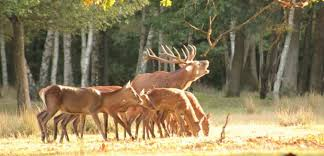
\includegraphics[width=.9\textwidth]{laRepro/CycleRepro.jpg}	
	\end{center}
	\caption{Grenouille à la recherche d'une partenaire!}%
	\label{fig:brameCerf}
\end{figure}

\subsection{La différenciation mâle/femelle}

Si le sexe est déterminé génétiquement, il est modulé par les conditions thermiques. 
Si l’hiver a été doux et bref, la production d’individus hermaphrodites augmente dans la population.
La différenciation sexuelle est postérieure à la métamorphose et a lieu lors de la croissance.
Le mâle possède une taille légèrement plus petite que la femelle.
La maturité sexuelle est acquise plus ou moins tardivement (en 3 ans pour la grenouille rousse). 
A partir de ce stade, en théorie, la croissance se poursuit lentement et indéfiniment. La grenouille vit en moyenne 5 ans, sa longévité maximale est de 15 ans.
        
\subsection{Le choix du partenaire}

En mars, les grenouilles sortent de leur hibernation.  
Dès que la température extérieure atteint environ 7deg C, les individus se mettent en route vers le site de reproduction, s’il n’était pas déjà sur place. 
Chez la plupart des espèces, l’accouplement a lieu dans l’eau.

Les femelles, encore à quelques kilomètres de distance, perçoivent le cri nuptial émis par leurs congénères grâce aux gonflements des sacs vocaux.


\begin{figure}
	\begin{center}
		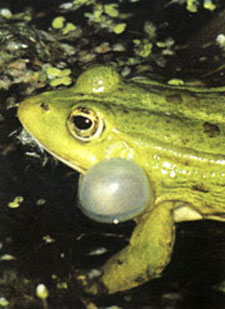
\includegraphics[width=.9\textwidth]{laRepro/sacvocal.jpg}
		\caption{Gonflement des sacs vocaux permettant l'émission de son.}%
		\label{fig:grossejoue}
	\end{center}
\end{figure}

Lorsque les femelles rejoignent le lieu d’accouplement, plusieurs mâles (parfois plus de 6) s’assemblent autour de chaque femelle. 
Dans certains cas, la qualité des vocalisations du mâle détermine le choix fait par la femelle. Cela est dangereux car cela peut attirer des prédateurs.

La femelle, reconnue avant tout par les phéromones qu’elle produit, est saisie par le mâle, qui glisse les bras sous ses aisselles. 
Pouce et avant-bras portent des callosités, les brosses copulatrices dont l’apparition (et la disparition après la reproduction) est contrôlée par les variations de sécrétion d’une hormone, la testostérone.
Le contact des brosses sur la peau de la femelle suscite un réflexe d’étreinte, soudant littéralement les deux partenaires. 
L’étreinte peut durer 7 jours ou plus. Les oeufs, expulsés du cloaque de la femelle, sont fécondés de manière externe par le mâle. La ponte finie, mâle et femelle se séparent.

 
\subsection{La ponte}

Les grenouilles européennes pondent de 1400 à 10 000 oeufs, d’un diamètre compris entre 1 et 3 mm. 
Chez certaines grenouilles américaines et tropicales, leur nombre peut dépasser 20 000 et le diamètre atteint 5 mm. 
Dotés d’un vitallus assez important, ils s’agglomèrent en de volumineuses masses gélatineuses.

Certaines grenouilles sont vivipares. 
Elles avalent alors leurs oeufs fécondés afin de les faire incuber dans l’estomac. 
Elles accouchent ensuite de petites grenouilles par la bouche. 
L’inhibition gastrique maintenue pendant toute la " gestation " est alors levée.

Cependant l’oviparité est le mode de reproduction le plus répandu. 
Chez certaines espèces, quand les oeufs sont en train d’éclore, le mâle se place au milieu, s’enduit de la gelée de la ponte et entre dans une torpeur progressive, pendant laquelle les têtards éclos sautent afin d’escalader son corps ; ils se placent ainsi dans les poches ventro-latérales qui s’étendent entre les deux paires de pattes et y finissent leur développement. 
De plus, quatre genres de grenouilles marsupiales ont développé une poche à oeuf dorsale.

         

\subsection{La croissance}

Le délai entre la fécondation et l’éclosion peut varier de 2 à 21 jours selon les espèces considérées. 
L’oeuf se développe en 3 phases qui dure de 3 à 4 mois. 
L’embryon âgé de quelques jours, doté d’une ventouse-suçoir et d’une queue esquissée, sort assez vite de la capsule gélatineuse l’enveloppant. 
C’est un têtard.

Incapable, de nager et de manger, le têtard se colle à la coque de l’oeuf ou à une feuille de plante aquatique. 
Sa bouche se forme, ses narines s’ouvrent puis les yeux apparaissent sous la peau. 
Sa queue s’allonge, tandis que, de chaque côté du cou, se distinguent des petites houppes ramifiées qui sont ces branchies externes.

Ce stade têtard prend fin en général au cours du 3ième mois mais la métamorphose proprement dite peut être différée de 2 ans dans certains milieux hostiles. 
La queue disparaît par autophagocytose et, rapidement, l’animal ne peut plus respirer sous l’eau (ses branchies disparaissent pendant que se développent les poumons).
Finalement, la petite grenouille fait son apparition sur la terre.

Ces 3 phases peuvent se dérouler exceptionnellement dans l’eau, l’éclosion donnant naissance à une grenouille presque entièrement formée. 
On observe ce phénomène chez certaines grenouilles de montagne dont l’environnement est défavorable et chez une famille de grenouilles de Nouvelle-Zélande.
        	
\begin{figure}%
	\begin{center}
	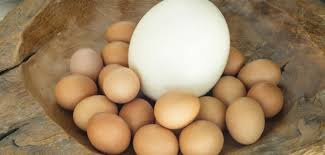
\includegraphics[width=.9\textwidth]{laRepro/oeuf.jpg}	
	\end{center}
	\caption{Exemple de grappe d'oeufs de rainettes.}%
	\label{fig:autruche}
		\end{center}

\end{figure}

Il existe des périodes sensibles du développement, pendant lesquelles peuvent se développer des malformations embryonnaires graves : moins de 1 des oeufs fécondés parviennent à l’âge adulte